\subsection{Zadania}

\setcounter{problem}{0}

\begin{problem}
  Załóżmy, że $\{X_n\}_{n\in\N}$ jest ciągiem niezależnych zmiennych losowych o takim samym rozkładzie, średniej $0$ i skończonej wariancji. Rozważmy filtrację $\mathds{F}=\{\set{F}_n\}$ zadaną przez $\set{F}_n=\sigma(X_0,X_1,...,X_n)$. Udowodnij, że ciąg
  $$Z_n=X_0X_1+X_1X_2+....+X_{n-1}X_n, \quad Z_0=0$$
  jest $\mathds{F}$-martyngałem.
\end{problem}

\begin{solution}
  {\color{red}Tak naprawdę to sprawdzenie że $Z_n$ są całkowalne powinno być na samym początku, bo inaczej to nie ma sensu.}

  Chcemy pokazać, że
  $$\expected{Z_{n+1}}{\set{F}_{n}}=Z_n$$
  dla dowolnego $n\in\N$.
  \begin{align*}
    \expected{Z_{n+1}}{\set{F}_n}&=\expected{Z_n+X_nX_{n+1}}{\set{F}_n}=\\ 
                                 &=\expected{Z_n}{\set{F}}+\expected{X_nX_{n+1}}{\set{F}_n}=\\ 
                                 &=Z_n+X_n\expected{X_{n+1}}{\set{F}_n}
  \end{align*}
  ponieważ $X_n$ jest $\set{F}_n$-mierzalne oraz
  $$\expected{|X_nX_{n+1}|}\leq\expected{X_n^2}^{1/2}\expected{X_{n+1}^2}^{1/2}<\infty$$
  gdzie nierówność wynika z nierówności Cauchy'ego-Schwarza, a $\expected{X_n^2}=Var(X_n)<\infty$.

  Zauważmy teraz, że $X_{n+1}$ jest niezależne od $\set{F}_n$, gdyż $X_n$ jest niezależne od każdej ze zmiennych $X_1,...,X_n$. W takim razie, $\expected{X_{n+1}}{\set{F}_n}=\expected{X_{n+1}}=0$, a więc ostatecznie dostajemy
  $$\expected{Z_{n+1}}{\set{F}_n}=Z_n+X_n\expected{X_{n+1}}{\set{F}_n}=Z_n+X_n\cdot 0=Z_n$$
  Czyli $Z_n$ faktycznie jest martyngałem.
\end{solution}

\begin{problem}
  Ustalmy $\theta\in\R$. Niech $X_1,X_2,...$ będzie ciągiem niezależnych zmiennych losowych o takim samym rozkładzie takich, że 
  $$\expected{e^{\theta X_1}}<\infty.$$
  Pokaż, że 
  $$M_n=\expected{e^{\theta X_1}}^{-n}\prod_{j=1}^ne^{\theta X_j}$$
  jest $\mathds{F}$-martyngałem dla filtracji $\mathds{F}=\{\set{F}_n\}$ danej przez $\set{F}_n=\sigma(X_1,...,X_n)$.
\end{problem}

\begin{solution}
  {\color{red}Tutaj ta sama uwaga co do poprzedniego zadania.}

  Zacznijmy od obserwacji, że
  $$M_{n+1}=\expected{e^{\theta X_1}}^{-n-1}\prod_{j=1}^{n+1}e^{\theta X_j}=M_n\cdot\expected{e^{\theta X_1}}^{-1}e^{\theta X_{n+1}}$$
  w takim razie, wwo $M_{n+1}$ to jest
  \begin{align*}
    \expected{M_{n+1}}{\set{F}_n}&=\expected{e^{\theta X_1}}^{-1}\cdot \expected{M_n\cdot e^{\theta X_{n+1}}}{\set{F}_n}
  \end{align*}
  Od razu widać, że $M_n$ jest mierzalne względem $\set{F}_n$, bo zależy tylko od zmiennych $X_1,...,X_n$ które $\set{F}_n$ generują. Chcemy teraz sprawdzić, czy $\expected{|M_n\cdot e^{\theta X_{n+1}}|}<\infty$, wówczas możemy wyciągnąć $M_n$ przed wwo.
  \begin{align*}
    \expected{|M_n\cdot e^{\theta X_{n+1}}|}&=\expected{\left |\expected{e^{\theta X_1}}^{-1}\cdot \prod_{j=1}^{n} e^{\theta X_j}\cdot e^{\theta X_{n+1}} \right| }=\\ 
                                            &=|\expected{e^{\theta X_1}}|^{-n}\cdot\expected{ \prod_{j=1}^{n+1}e^{\theta X_j} }=\\ 
                                            &=|\expected{e^{\theta X_1}}|^{-n}\cdot \prod_{j=1}^{n+1}\expected{e^{\theta X_j}}=\\ 
                                            &=\expected{e^{\theta X_{n+1}}}=\expected{e^{\theta X_1}}<\infty
  \end{align*}
  ponieważ jeśli $\{X_n\}$ są niezależne, to $e^{X_n}$ też są niezależne, a dla niezależnych $X,Y$ zachodzi $\expected{XY}=\expected{X}\expected{Y}$.
  W takim razie dostajemy
  $$\expected{M_{n+1}}{\set{F}_n}=\expected{e^{\theta X_1}}^{-1}\expected{M_n\cdot e^{\theta X_{n+1}}}{\set{F}_n}=M_n\expected{e^{\theta X_1}}^{-1}\expected{e^{\theta X_{n+1}}}{\set{F}_{n}}$$
  ale ponieważ $\set{F}_n$ nie zawiera ani grama informacji o $X_{n+1}$, to $e^{\theta X_{n+1}}$ jest niezależne od $\set{F}_n$, więc
  $$\expected{e^{\theta X_{n+1}}}{\set{F}_n}=\expected{e^{\theta X_{n+1}}}=\expected{e^{\theta X_1}}$$
    a to już daje to co chcieliśmy.
\end{solution}

\begin{problem}
  Niech $\{Y_n\}$ będzie ciągiem niezależnych zmiennych losowych o średniej $0$ i wariancji $\sigma^2$. Pokaż, że ciąg 
  $$X_n=\left(\sum_{k=1}^nY_k\right)^2-n\sigma^2$$
  jest martyngałem.
\end{problem}

\begin{solution}
  {\color{red}Tutaj powinniśmy sprawdzić jeszcze $\mathds{F}$-adaptowalność $\{X_n\}$ i jego całkowalność.}

  Zacznijmy od wyrażenia $X_{n+1}$ przy użyciu $X_n$
  \begin{align*}
    X_{n+1}&=\left( \sum_{k=1}^{n+1}Y_{k} \right)^2 - (n+1)\sigma^2= \left( \sum_{k=1}^nY_k +Y_{n+1} \right)^2 - (n+1)\sigma^2=\\ 
           &=\left(\sum_{k=1}^n Y_k \right)^2 -n\sigma ^2 + 2 Y_{n+1}\left( \sum_{k=1}^n Y_k \right) +Y_{n+1}^2 -\sigma^2=\\ 
           &=X_n+2\left( \sum_{k=1}^nY_{n+1}Y_k \right) -\sigma^2 + Y_{n+1}^2
  \end{align*}
  Rozważmy teraz filtrację $\mathds{F}=\{\set{F}_n\}$ dla ciągu $\set{F}_n=\sigma(Y_1,...,Y_n)$. Wtedy mamy
  \begin{align*}
    \expected{X_{n+1}}{\set{F}_n}&=\expected{X_n+2 \left( \sum_{k=1}^nY_{n+1}Y_k \right) -\sigma^2+Y_{n+1}^2}{\set{F}_n}=\\
                                 &=\expected{X_n}{\set{F}_n}+2\sum\expected{Y_{n+1}Y_n}{\set{F}_n}-\sigma^2+\expected{Y_{n+1}^2}{\set{F}_n}=(\star)
  \end{align*}
  Zmienna $X_n$ jest $\set{F}_n$-mierzalna bo korzysta tylko z informacji zapisywanych przez $Y_1,...,Y_n$. Zmienna $Y_{n+1}$ jest niezależna od $\set{F}_n$, bo zmienne $\{Y_n\}$ są niezależne. Zmienna $Y_{n+1}Y_k$ jest całkowalna dla dowolnego $k$, bo $\expected{|Y_{n+1}Y_k|}=\expected{|Y_{n+1}|}\expected{|Y_k|}=0$. W takim razie wracając do równości wyżej, można napisać
  \begin{align*}
    (\star)&=X_n+2\sum Y_{k}\expected{Y_{n+1}}{\set{F}_n}-\sigma^2+\expected{Y_{n+1}^2}=\\ 
           &=X_n+2\sum Y_k\expected{Y_{n+1}}-\sigma^2+\sigma^2=X_n+2\sum Y_k\cdot 0=X_n
  \end{align*}
  W takim razie ciąg $\{X_n\}$ jest $\mathds{F}$-martyngałem.
\end{solution}

\begin{problem}
  Niech $\{X_n\}$ będzie $\mathds{F}$-martyngałem. Pokaż, że dla każdych naturalnych $m,n$
  $$\expected{X_{m+n}}{\set{F}_n}=X_n.$$
\end{problem}

\begin{solution}
  Dla $m=1$ działa z definicji martyngału.

  Zakładamy teraz, że $\expected{X_{m+n}}{\set{F}_n}=X_n$ i chcemy to samo dostać dla $m+1$ (indukcja).

  Z własnośći wwo \ref{o arytmetyce wwo} wiemy, że jeśli mamy dwa zawarte w sobie $\sigma$-ciała $\set{G}_1\subseteq\set{G}_2$, to
  $$\expected{\expected{X}{\set{G}_2}}{\set{G}_1}=\expected{X}{\set{G}_1}$$
  tutaj bierzemy $\set{G}_1=\set{F}_n$ natomiast $\set{G}_2=\set{F}_{n+m}$. Mamy więc
  $$\expected{\expected{X_{m+n+1}}{\set{F}_{m+n}}}{\set{F}_n}=\expected{X_{m+n+1}}{\set{F}_n}$$
  Z faktu, że $\{X_n\}$ jest martyngałem to mamy
  $$\expected{X_{m+n+1}}{\set{F}_{n+m}}=X_{m+n}$$
  czyli przechodząc już do sedna sprawy,
  \begin{align*}
    \expected{X_{m+n+1}}{\set{F}_n}&=\expected{\expected{X_{m+n+1}}{\set{F}_{m+n}}}{\set{F}_n}=\\ 
                                   &=\expected{X_{m+n}}{\set{F}_n}=X_n
  \end{align*}
  bo ostatnie przejście wynika z założenia indukcyjnego.
\end{solution}

\begin{problem}
  Niech $\{X_n\}$ będzie nadmartyngałem takim, że $\expected{X_n}=\expected{X_0}<\infty$ dla każdego $n\in\N$. Pokaż, że $\{X_n\}$ jest martyngałem.
\end{problem}

\begin{solution}
  Nadmartyngał spełnia
  $$\expected{X_{n+1}}{\set{F}_n}\leq X_n$$
  Po pierwsze zauważmy, że
  $$\expected{X_n-\expected{X_{n+1}}{\set{F}_n}}=\expected{X_n}-\expected{\expected{X_{n+1}}{\set{F}_n}}=\expected{X_n}-\expected{X_{n+1}}=0,$$
  czyli $\expected{X_n-\expected{X_{n+1}}{\set{F}_n}}=0$, a ponieważ z warunku na nadmartyngał $X_n-\expected{X_{n+1}}{\set{F}_n}\geq0$ prawie wszędzie, to mamy nieujemną funkcję której całka jest $0$ $\implies$ ta funkcja jest prawie wszędzie równa zero.
\end{solution}

\begin{problem}
  Pokaż, że jeżeli $T_1,T_2$ są czasami zatrzymania, to $\min\{T_1,T_2\}$ i $\max\{T_1,T_2\}$ również są czasami zatrzymania. Czy $T_1^2, T_1+1,T_1+T_2, T_1-1, \min\{T_1,2T_2\}$ są też czasami zatrzymania?
\end{problem}

\begin{solution}
  Przychodzimy do tego zadania z wiedzą, że zdarzenie $\{T_i=n\}$ jest w zbiorze $\set{F}_n$ dla dowolnego $n$. Od razu zauważmy, że skoro $\set{F}_1\subseteq\set{F}_2\subseteq...$, to jeśli $\{T_i=n\}\in\set{F}_n$ dla dowolnego $n$, to $\set{F}_n$ nadal trzyma informację o $\{T_i=k\}$ dla $k\leq n$, czyli możemy równoważnie powiedzieć, że $\{T_i\leq n\}\in\set{F}_n$.

  Zdarzenie $\{\max\{T_1,T_2\}\leq n\}$ jest równoważne zdarzeniu 
  $$\{\max\{T_1,T_2\}\leq n\}=\{T_1\leq n\;i\;T_2\leq n\}=\{T_1\leq n\}\cap \{T_2\leq n\}$$
  a ponieważ $\set{F}_n$ jest $\sigma$-ciałem, to skoro dwa zbiory do niego należą, to należeć też musi ich przekrój.

  Zdarzenie $\{\min\{T_1,T_2\}=n\}$ potencjalnie pyta o czas w nieskończonej przyszłości, bo możemy je zapisać jako
  $$\min\{T_1, T_2\}=n\iff (T_1=n\;\land T_2\geq n)\;\lor\;(T_1\geq n\;\land\; T_2=n)$$
  ale jeśli popatrzymy na zdarzenie
  $$\{\min\{T_1,T_2\}\leq n\}=\{T_1\leq n\;lub\;T_2\leq n\}=\{T_1\leq n\}\cup \{T_2\leq n\}$$
  wiemy, że oba składniki tej sumy są w $\set{F}_n$, więc i cała suma w $\set{F}_n$ siedzi.

  \begin{enumerate}
    \item $T_1^2$ jest czasem zatrzymania, bo
      $$\{T_1^2\leq n\}=\{T_1\leq\sqrt{n}\leq n\}$$
      jest elementem $\set{F}_n$.
    \item $T_1+1$ jest czasem zatrzymania, bo
      $$\{T_1+1= n\}=\{T_1= n-1\}$$
      co w oczywisty sposób daje nam $\{T_1=n-1\}\in\set{F}_{n-1}\subseteq\set{F}_n$
    \item $T_1+T_2$ jak najbardziej jest czasem zatrzymania, bo dla $i\neq j$ zbiory $\{T_1=i\;\land\;T_2=n-i\}$ oraz $\{T_1=j\;\land\;T_2=n-j\}$ są rozłączne, a więc
      $$\{T_1+T_2=n\}=\bigcup_{k\leq n}\{T_1=k\;i\;T_2=n-k\}$$
      każdy element sumy należy do $\set{F}_n$ jak przekrój dwóch jego elementów, więc i cała suma do niego należy.
    \item $T_1-1$ nie koniecznie jest czasem zatrzymania, bo
      $$\{T_1-1=n\}=\{T_1=n+1\}$$
      może należeć tylko do $\set{F}_{n+1}$, ale nie trafiać w $\set{F}_n$. Rozważmy choćby modelowanie gry w której wygrywamy i przegrywamy dolara z takim samym prawdopodobieństwem (wykład następny), ale dorzućmy możliwość nie obstawiania, czyli "kroku 0". Załóżmy, że startujemy z zerem dolarów. Innymi słowy, rozważamy skakanie w losowy sposób po $\Z$ z możliwością podskoczenia tylko pionowo w górę. Wtedy jeśli $X_i$ będzie naszym aktualnym położeniem na $\Z$ po $i$ krokach, a $\set{F}_i=\sigma(X_1,...,X_i)$, to $\set{F}_1$ będzie posiadało tylko informację o zdarzeniu $\{X_1=-1\}$, $\{X_1=0\}$ i $\{X_1=1\}$, a więc gdy $T_1=\inf\{n\;:\;X_n=1\}$, to zdarzenie
      $$\{T_1-1=1\}=\{T_1=2\}=\{X_1=1\}\cup \{X_1=0\;i\;X_2=1\}$$
      należy do $\set{F}_2$, ale do $\set{F}_1$ już należeć nie ma możliwości.
  \end{enumerate}
\end{solution}

\begin{problem}
  Niech $T$ będzie czasem zatrzymania. Załóżmy, że istnieje $\varepsilon\in(0,1)$ oraz $N\in\N$ takie, że
  $$\prob{T\leq N+n}{\set{F}_n}>\varepsilon$$
  dla każdego $n\in\N$. Pokaż, że $\expected{T}<\infty$.
\end{problem}

\begin{solution}
  Zaczniemy od obserwacji, że
  \begin{align*}
    \expected{T}&=\sum_{n\geq0}n\prob{T=n}=\sum_{n\geq0}\sum_{k=0}^{n-1}\prob{T=n}=\sum_{n\geq0}\prob{T>n}
  \end{align*}
  \begin{center}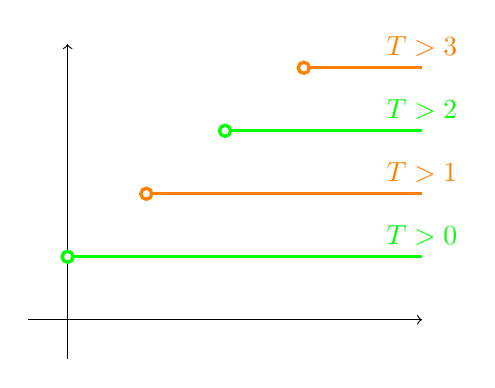
\begin{tikzpicture}
    \draw[->] (-0.5, 0)--(4.5, 0);
    \draw[->] (0, -0.5)--(0, 3.5);

    \draw[green, very thick] (0, 0.8)--(4.5, 0.8) node [above] {$T>0$};
    \draw[orange, very thick] (1, 1.6)--(4.5, 1.6) node [above] {$T>1$};
    \draw[green, very thick] (2, 2.4)--(4.5, 2.4) node [above] {$T>2$};
    \draw[orange, very thick] (3, 3.2)--(4.5, 3.2) node [above] {$T>3$};
    
    \filldraw[color=green, fill=white, very thick] (0, 0.8) circle (2pt);
    \filldraw[color=orange, fill=white, very thick] (1, 1.6) circle (2pt);
    \filldraw[color=green, fill=white, very thick] (2, 2.4) circle (2pt);
    \filldraw[color=orange, fill=white, very thick] (3, 3.2) circle (2pt);
  \end{tikzpicture}\end{center}
  Będziemy chcieli oszacować całe to wyrażenie od góry przez zbieżny szereg. Dokładnie, będzie nam potrzebne oszacowanie go przez $\prob{T>kN}$:
  $$\expected{T}=\sum_{n\geq 0}\prob{T>n}=\sum_{k\geq 0}\sum_{n=kN}^{(k+1)N-1}\prob{T>n}\leq \sum_{k\geq 0}N\cdot\prob{T>kN}\;(\text{\Coffeecup})$$
  gdyż funkcja $\prob{T>n}$ jest malejąca, a więc przyjmuje ekstremum na lewym krańcu. Dzielimy więc $\sum\prob{T>n}$ na odcinki $[kN, (k+1)N)$ i szacujemy sumę na każdym z nich przez $N\cdot \prob{T>kN}$.

  Żeby jednak dokończyć szacowanie wyżej, potrzebujemy ograniczyć $\prob{T>kN}$ od góry. Z definicji prawdopodobieństwa warunkowego wiemy, że
  $$1\geq\prob{T\leq N+n}{\set{F}_n}=\expected{\mathds{1}_{\{T\leq N+n\}}}{\set{F}_n}>\varepsilon$$
  Funkcja $\mathds{1}_{\{T\leq N+n\}}=1-\mathds{1}_{\{T>N+n\}}$, więc mamy
  $$1\geq \expected{1-\mathds{1}_{\{T>N+n\}}}{\set{F}_n}=\expected{1}{\set{F}_n}-\expected{\mathds{1}_{\{T>N+n\}}}{\set{F}_n}=1-\expected{\mathds{1}_{\{T>N+n\}}}{\set{F}_n}>\varepsilon$$
  Po przerzuceniu $\varepsilon$ na lewą stronę, a wwo na prawą stronę, dostajemy
  $$1-\varepsilon > \expected{\mathds{1}_{\{T>N+n\}}}{\set{F}_n}\quad(\star)$$
  co po nałożeniu całki na obie strony implikuje, że
  $$1-\varepsilon>\expected{\mathds{1}_{\{T>N+n\}}}=\prob{T>N+n}$$

  Wróćmy do punktu $(\star)$ i rozważmy zdarzenie 
  $$G=[\{T\leq n\}]^c=\{T>n\}\in\set{F}_n.$$ 
  Zdarzenie $\{T\leq n\}\in\set{F}_n$, bo $T$ jest czasem zatrzymania, a jego dopełnienie należy do tego zbioru ze względu na fakt, że $\set{F}_n$ jest $\sigma$-ciałem. Jeśli nałożymy na obie strony $(\star)$ całkowanie po $G$, to dostajemy
  \begin{align*}
    \prob{T>n}(1-\varepsilon)&=\\=(1-\varepsilon)\expected{\mathds{1}_G}&=\\={\color{blue}\expected{(1-\varepsilon)\mathds{1}_G}}&{\color{blue}>\expected{\expected{\mathds{1}_{\{T> N+n\}}}{\set{F}_n}\mathds{1}_G} }=\\ 
                                                                                  &=\expected{\mathds{1}_{\{T> N+n\}}\mathds{1}_G}=\expected{\mathds{1}_{\{T>N+n>n\}}}=\\ 
                                                                                  &=\prob{T>N+n}
  \end{align*}
  Dostaliśmy więc
  $$\prob{T>n}(1-\varepsilon)>\prob{T>N+n}$$
  Niech teraz $n=k\cdot N$. Wtedy
  \begin{align*}
    \prob{T>(k+1)N}=\prob{N+kN}&<\\
    <\prob{T>k\cdot N}(1-\varepsilon)&=\\ 
    = {\color{red}\prob{T>n}}(1-\varepsilon)&=\prob{T>N+(k-1)N}(1-\varepsilon)<\\ 
                                                                             &<(1-\varepsilon)(1-\varepsilon)\prob{T>(k-1)N}.
  \end{align*}
  a w szczególności gdy $n=0$, to $\prob{T>1\cdot N}<(1-\varepsilon)^1=1-\varepsilon$. Sugeruje to, że zachodzi wzór% (udowadniany indukcyjnie tak jak w równości wyżej)
  $$(1-\varepsilon)^k>\prob{T>k\cdot N}$$
  który udowadniamy indukcyjnie. Dla $k=0$ sprawa jest oczywista, a dla kroku indukcyjnego $k\implies k+1$ zaczynamy od góry i kontynuujemy jak w nierówności wyżej aż do czerwonego $\prob{T>n}$.

  Wróćmy teraz do $(\text{\Coffeecup})$ i dokończmy szacowanie $\expected{T}$
  $$\expected{T}\leq \sum_{k\geq 0}N\prob{T>kN}\leq N\sum_{k\geq 0}(1-\varepsilon)^k\leq N\sum e^{-k\varepsilon}<\infty$$
\end{solution}
